% Figure: the planned place of the persistence layer between the modeling tools
% and a local IPFS node. Standalone TikZ source, colors as in the manuscript.
\documentclass[tikz,border=2pt]{standalone}
\usepackage[T1]{fontenc}
\usepackage{newtxtext}
\usetikzlibrary{arrows.meta,calc}

\definecolor{ink}{HTML}{0B0B0B}
\definecolor{inksoft}{HTML}{52514E}
\definecolor{mutedfill}{HTML}{F0EFEC}
\definecolor{newfill}{HTML}{CDE2FB}
\definecolor{newborder}{HTML}{1C5CAB}

\begin{document}
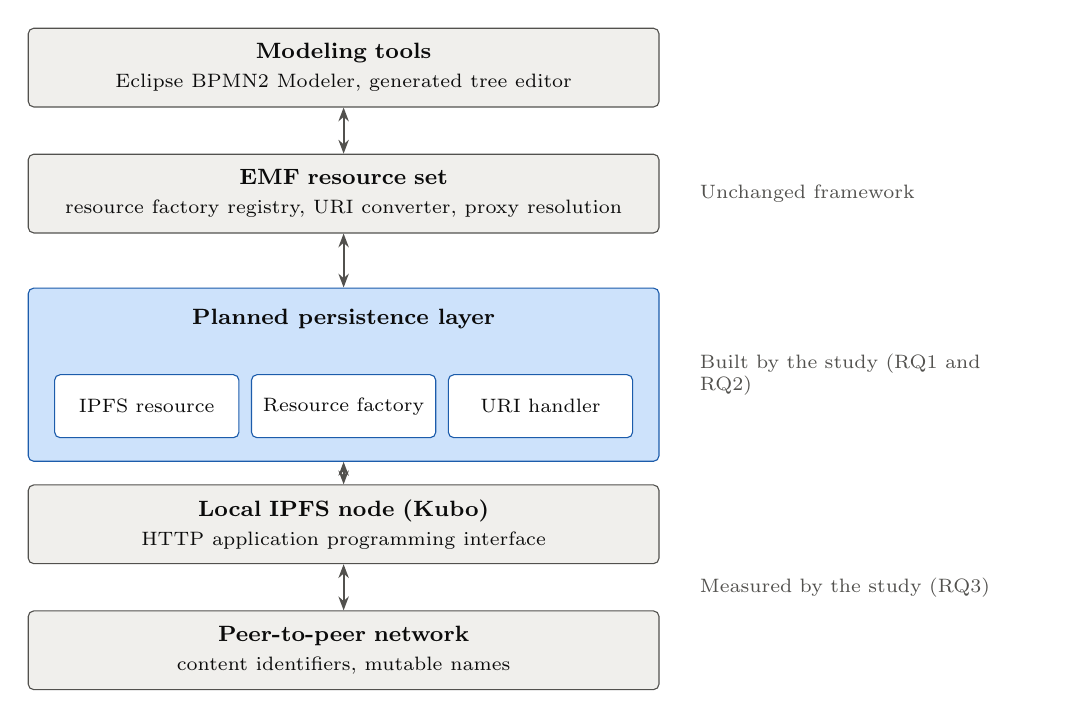
\begin{tikzpicture}[
  font=\footnotesize,
  >={Stealth[length=5pt]},
  layer/.style={draw=inksoft, fill=mutedfill, rounded corners=2pt, text=ink,
    align=center, text width=78mm, minimum height=10mm, inner sep=3pt},
  newlayer/.style={layer, fill=newfill, draw=newborder},
  part/.style={draw=newborder, fill=white, rounded corners=2pt, text=ink,
    align=center, text width=22mm, minimum height=8mm, inner sep=2pt, font=\scriptsize},
  link/.style={<->, draw=inksoft, line width=0.7pt},
  side/.style={text=inksoft, font=\scriptsize, align=left, anchor=west, text width=42mm}
]

\node[layer] (tools) at (0,0) {\textbf{Modeling tools}\\[1pt]\scriptsize Eclipse BPMN2 Modeler, generated tree editor};
\node[layer] (emf) at (0,-16mm) {\textbf{EMF resource set}\\[1pt]\scriptsize resource factory registry, URI converter, proxy resolution};
\node[newlayer, minimum height=22mm] (plugin) at (0,-39mm) {};
\node[anchor=north, text=ink] at ($(plugin.north)+(0,-1.5mm)$) {\textbf{Planned persistence layer}};
\node[part] at (-25mm,-43mm) {IPFS resource};
\node[part] at (0mm,-43mm) {Resource factory};
\node[part] at (25mm,-43mm) {URI handler};
\node[layer] (node) at (0,-58mm) {\textbf{Local IPFS node (Kubo)}\\[1pt]\scriptsize HTTP application programming interface};
\node[layer] (net) at (0,-74mm) {\textbf{Peer-to-peer network}\\[1pt]\scriptsize content identifiers, mutable names};

\draw[link] (tools) -- (emf);
\draw[link] (emf) -- (plugin);
\draw[link] (plugin) -- (node);
\draw[link] (node) -- (net);

\node[side] at (44mm,-16mm) {Unchanged framework};
\node[side] at (44mm,-39mm) {Built by the study (RQ1 and RQ2)};
\node[side] at (44mm,-66mm) {Measured by the study (RQ3)};
\end{tikzpicture}
\end{document}
